\documentclass[12pt]{article}
\usepackage[utf8]{inputenc}
\usepackage[russian]{babel}
\usepackage{hyperref}
\usepackage{color}
\usepackage{amssymb}
\usepackage{amsmath}
\usepackage{graphicx}
\usepackage{tikz}
\usepackage{titling}
\usepackage{lipsum}
\usepackage{titlesec}

\titlespacing\section{0pt}{10pt plus 2pt minus 2pt}{0pt plus 2pt minus 2pt}

\setlength{\droptitle}{-10em}   % This is your set screw

\author{Михаил Лепехин и Роман Логинов, группа 694}
\title{Online Convex Optimization (OCO)}

\begin{document}
  \maketitle

\section*{Применение Online Convex Optimisation к задаче фильтрации спама}
$ $

Предположим, что признаки email-сообщений принадлежат множеству $\mathcal{X}$. В качестве признаков будем рассматривать частоты вхождений слов (или групп слов, чтобы размерность мн-ва признаков не получилась слишком большой) в сообщение.

На каждом шаге $t$ функция $a_t : \mathcal{X} \rightarrow [0, 1]$, сопоставляет вектору $x \in \mathcal{X}$ значений признаков некоторое число из отрезка $[0, 1]$. По смыслу это значение является оценкой вероятности (уверенности) того, что сообщение с данными значениями признаков является спамом.

На каждом шаге $t$ соперник выбирает вектор значений признаков $x_t$ и индикатор $y_t$ того, что данное сообщение является спамом.

Для оценки точности метода принятия решений $a_t$ нужно взять некоторую функцию потерь $f_t$. Например, квадратичную функцию потерь:

$$f_t(a_t) := (y_t-a_t(x_t))^2.$$

На каждом шаге функция $a_t(x)$ выбирается из некоторого множества так, чтобы минимизировать $regret$:

$$\sum\limits_{t=1}^T f_t(a_t) - \min\limits_{a \in \mathcal{A}} \sum\limits_{t=1}^T f_t(a) = \sum\limits_{t=1}^T (y_t-a_t(x_t))^2 - \min\limits_{a \in \mathcal{A}} \sum\limits_{t=1}^T (y_t-a(x_t))^2$$

\section*{Выбор функции $a_t(x)$}
$ $


В машинном обучении для решения задачи классификации спама часто делают следующее. При помощи некоторого алгоритма находят вектор фильтра $a$ из шара $B_R(0)$ относительно некоторой нормы. А после - для определения, является ли сообщение с вектором значений признаков $x$ спамом, рассматривают скалярное произведение $<a, x>$.

Если $<a, x>$ > 0, то сообщение является спамом. Если же знак скалярного произведения отрицательный, то сообщение не является спамом. А если получилось так, что скалярное произведение равно 0, то считается, что тип сообщения не определён.

Будем строить функцию $a_t$ из похожих соображений. Будем также подбирать вектор фильтра $w_t$ из $W := B_R(0)$ и большим значениям скалярного произведения $<w_t, x>$ будет сопоставлять большую вероятность.

В качестве $\mathcal{X}$ возьмём множество векторов $x$ из $\mathbb{R_{+}}^d$, что $\sum\limits_{i=1}^n x_i = 100$ (здесь каждой группе слов сопоставляется процент количества слов из этой группы по отношению ко всем словам в сообщении).

Покажем, что скалярного произведение $<w_t, x>$ ограничено. По неравенству Коши-Буняковского:

$$<w_t, x>^2 \leq ||w_t||_2^2*||x||_2^2 \leq R^2*||x||_2^2 \leq R^2*100^2.$$

Причём, равенство здесь достигается, если сразу выполняются 3 ограничения:

1) $x$ коллинеарен $w_t$ - получим равенство в нер-ве К-Б,

2) $w_t=R$ - получим 2 равенство,

3) $\exists i \in \{1, \dots, d\}: x_i = 100$.

Тогда определим $M := 100R$.

В качестве функции $a_t(x)$ возьмём

 $$a_t(x) = \frac{<x, w_t>+M}{2M}.$$
 
 Тогда функция $f_t$ запишется следующим образом:
 
 $$f_t(x) = \bigg(y_t - \frac{<x, w_t>+M}{2M}\bigg)^2$$
 
\section*{Свойства выбранной функции $a_t(x)$}
$ $

Для нас очень важным свойством будет являться то, что выбранная функция $a_t(x)$ выпукла. Покажем это.

Вычислим её градиент.

$$\frac{\partial f_t}{\partial x}(x) = \frac{2}{2M}(<x, w_t>+M)\frac{w_t}{2M} = \frac{<x, w_t>+M}{4M^2}w_t$$

Продифференцируем градиент по $x$ и получим гессиан.

$$\frac{\partial^2 f_t}{\partial x^2}(x) = \frac{1}{4M^2}w_tw_t^T \succeq 0$$

Положительная полуопределённость следует из того, что $\forall x \in \mathcal{X}: x^Tw_tw_t^Tx_t = (w_t^Tx_t)^Tw_t^Tx_t = <w_t^Tx_t, w_t^Tx_t> \geq 0$ - по свойствам скалярного произведения.

По дифференциальному критерию выпуклости 2 порядка функция $f_t(x)$ выпукла. 

\section*{Вычисление regret}
$ $

Для того, чтобы проверять качество работы методов, очень полезно уметь получать значение $regret$.

С учётом выбора функции $a_t(x)$ $regret$ можно записать следующим образом:

$$\sum\limits_{t=1}^T (y_t-a_t(x_t))^2 - \min\limits_{a \in \mathcal{A}} \sum\limits_{t=1}^T (y_t-a(x_t))^2 =$$
$$= \sum\limits_{t=1}^T\bigg(y_t - \frac{<x_t, w_t>+M}{2M}\bigg)^2 - \min\limits_{w \in W}\sum\limits_{t=1}^T\bigg(y_t - \frac{<x_t, w>+M}{2M}\bigg)^2$$

При этом заметим, что $\forall t=1, \dots, T: g_t(w) = \bigg(y_t - \frac{<x_t, w>+M}{2M}\bigg)^2$ является выпуклой по $w$ (доказательство аналогично выпуклости $f_t$ по $x$).
Значит, функция $g(w) = \sum\limits_{t=1}^T\bigg(y_t - \frac{<x_t, w>+M}{2M}\bigg)^2$ является выпуклой как сумма выпуклых функций.

Чтобы получить точное или приближённое значение $regret$ нужно точно или приближённо решить следующую задачу оптимизации:

$$\min g(w)$$
$$s.t. w \in W$$

Эта задача является выпуклой, поскольку:

1) $g(w)$ выпукла в $\mathbb{R}^d$, как было показано выше;

2) множество $W = B_0(R)$ выпукло, поскольку любые 2 точки, лежащие в шаре можно соединить отрезком, каждая точка которого будет также принадлежать этому шару.


Поэтому для получения точного значения $regret$ можно применить теорему Каруша-Куна-Таккера. В силу выпуклости задачи  оптимизации стационарные точки лагранжиана будут точками минимума функции. 

Но нам вполне хватит и приближённого означения $regret$, поэтому для решения вспомогательной задачи оптимизации воспользуемся пакетом $cvxpy$.

\section*{Методы первого порядка}
$ $

В данном разделе мы рассмотрим базовые алгоритмы для Online Convex Optimization, которые достаточно неплохо применимы на практике.

В целом данные методы похожи на соответствующие методы первого порядка для задач обычной выпуклой оптимизации. Но они принципиально отличаются целью применения. Ведь при помощи методов OCO мы стремимся минимизировать не ошибку оптимизации, а \textit{regret}:

$$regret = \sum\limits_{t=1}^T f_t(x_t) - \min\limits_{x \in \mathcal{K}} \sum\limits_{t=1}^T f_t(x)$$

Для сравнения $regret$ с ошибкой оптимизации полезно рассмотреть среднее значение $regret$, т.е. $\frac{regret}{T}$.

Введём обозначение:

$$\overline{x}_T := \frac{1}{T}\sum\limits_{t=1}^T x_t$$

Пусть все функции $f_t$ равны некоторой функции $f : \mathcal{K} \rightarrow \mathbb{R}$, то из неравенства Йенсена получим:

$$f(\overline{x}_T)-f(x^*) = f(\overline{x}_T)- \frac{1}{T} \sum\limits_{t=1}^T f(x^*) \leq \frac{1}{T}\sum\limits_{t=1}^T \big(f(x_t)-   f(x^*)\big	)$$

Таким образом мы показали следующий факт: 

функция $f(x_T)$ сходится к $f(x*)$ не менее быстро, чем среднее значение $regret$.

\section*{Online gradient descent}
$ $

Этот алгоритм, пожалуй, является одним из наиболее интуитивных и простых в Online Convex Optimization. Он базируется на известном нам методе градиентного спуска для offline выпуклой оптимизации.

На каждой итерации этот алгоритм делает шаг от предыдущей точки $x_k$ в направлении градиента предыдущего веса. Но такой шаг может привести к выходу за границу допустимого выпуклого множества $D$. Для того, чтобы этого не произошло, алгоритм проецирует полученную точку обратно на множество $D$, находя ближайшую к ней в $D$.

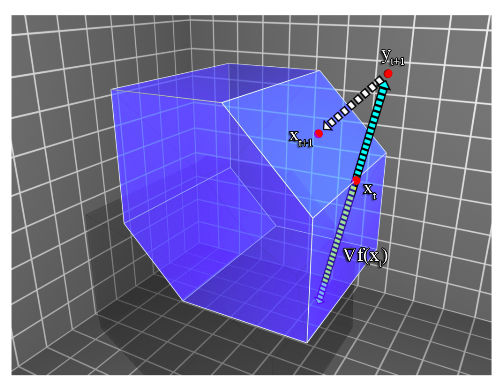
\includegraphics[width=\linewidth]{gradient_descent.png}

Несмотря на то, что функция весов на следующем шаге может существенно отличаться от веса на предыдущем шаге, $regret$, получаемый алгоритмом все равно будет сублинейным.

Это следует из следующей теоремы.

\textbf{Теорема.} Online градиентный спуск с шагом, заданным по правилу $\alpha_t = \frac{D}{G\sqrt{t}}$, для любого $T \geq 1$ гарантирует:

$$regret = \sum\limits_{t=1}^T f_t(x_t) - \min\limits_{x\in \mathcal{K}} \sum\limits_{t=1}^T f_t(x) \leq \frac{3}{2}GD\sqrt{T}$$

Кроме того, при выборе шага по данному правилу метод online градиентного спуска является асимптотически оптимальным по значению $regret$.

\textbf{Теорема.} Любой алгоритм для OCO в худшем случае выдаёт $regret = \Omega(DG\sqrt{T})$. Это утверждение верно даже при выборе функции веса из некоторого фиксированного распределения.

\section*{Stochastic gradient descent}
$ $
\end{document}